%============================================================
% CH1 · LESSON 2 — INDICES AND RANGES
%============================================================
\subsection{Indices and Ranges: Writing Loops Without Off-by-One Errors}
\label{ssec:ch1-indices}

Most wrong answers on easy array problems are not wrong ideas: they are a loop that runs one step too far, a range that misses its last element, or a comparison with a neighbour that does not exist. This lesson fixes one convention for ranges, shows why it removes most of these bugs, and gives you a tool --- the \emph{loop invariant} --- to convince yourself that a loop is right before you run it.

%------------------------------------------------------------
\subsubsection*{1. 0-based and 1-based indices}

C++ arrays are \textbf{0-based}: the $n$ elements are \texttt{a[0]}, \ldots, \texttt{a[n-1]} (Lesson~\ref{ssec:ch1-array} explains why). Problem statements, on the other hand, usually number positions $1..n$ (``$a_1, a_2, \dots, a_n$''). You can handle this in two ways, and both are fine as long as you pick one per program and stick to it:

\begin{table}[H]
\centering\small
\renewcommand{\arraystretch}{1.2}
\begin{tabularx}{\linewidth}{@{}>{\raggedright\arraybackslash}p{3.5cm} X X@{}}
\toprule
 & \textbf{convert to 0-based} & \textbf{keep 1-based} \\
\midrule
storage & \texttt{vector<int> a(n)}, read into \texttt{a[0..n-1]} & \texttt{vector<int> a(n + 1)}, read into \texttt{a[1..n]}, \texttt{a[0]} unused \\
statement says ``position $p$'' & use \texttt{a[p - 1]} & use \texttt{a[p]} \\
printing a position & print \texttt{i + 1} & print \texttt{i} \\
good for & LeetCode, library functions, \texttt{\%} arithmetic (Pattern~4) & prefix sums with $P[0] = 0$ (Chapter~\ref{ch:prefix_sums}), formulas copied from the statement \\
\bottomrule
\end{tabularx}
\end{table}

\begin{warningbox}[Mixing the two conventions]
The classic bug: read into \texttt{a[1..n]} but loop \texttt{for (int i = 0; i < n; i++)} --- the loop reads the unused \texttt{a[0]} and never reads \texttt{a[n]}. Decide the convention at the line that reads the input, and write it in a comment.
\end{warningbox}

%------------------------------------------------------------
\subsubsection*{2. Half-open ranges $[l, r)$}

A \textbf{range} is a set of consecutive positions. There are four ways to write one, and this book uses one of them everywhere:

\begin{definitionbox}[Half-open range]
$\seg{l}{r}$ denotes the positions $l, l+1, \dots, r-1$: the left end is \emph{included}, the right end is \emph{excluded}. Its length is $r - l$, and it is empty exactly when $l = r$.
\end{definitionbox}

\begin{diagrambox}
\begin{tikzpicture}
    \dpindex{hi}{-0.05}{$i$}{0}{7}
    \dparray{h}{0.6}{\texttt{a}}{5/acell, 2/awin, 8/awin, 1/awin, 9/acell, 3/acell, 6/acell, 4/acell}
    \aptrup{h1}{l = 1}{successgreen}
    \aptrup{h4}{r = 4}{accentorange}
    \arange{hi1}{hi3}{$[1, 4)$: $r - l = 3$ elements}{memoorange}
    \node[note, anchor=west, text width=4.4cm, align=left] at (7.5,0.6)
        {$r$ points \emph{just past} the last element.\\ The whole array is $[0, n)$.\\ $[4, 4)$ is empty.};
\end{tikzpicture}
\figcap{The range $[1, 4)$ covers \texttt{a[1]}, \texttt{a[2]}, \texttt{a[3]} --- three cells, and $4 - 1 = 3$.}
\end{diagrambox}

Why half-open? Because every everyday operation becomes formula-free:
\begin{itemize}[leftmargin=*]
    \item \textbf{Length} is $r - l$, with no ``$+1$''.
    \item \textbf{The loop} is always \texttt{for (int i = l; i < r; i++)}, and the whole array is \texttt{for (int i = 0; i < n; i++)} --- the familiar loop \emph{is} the half-open range $[0, n)$.
    \item \textbf{Splitting} $[l, r)$ at any $m$ with $l \le m \le r$ gives $[l, m)$ and $[m, r)$: no overlap, no gap, no $m \pm 1$.
    \item \textbf{Empty ranges} need no special case: $[l, l)$ has length $0$ and its loop runs zero times.
    \item The C++ library speaks the same language: \texttt{sort(a.begin() + l, a.begin() + r)} sorts $[l, r)$, and \texttt{a.end()} points just past the last element.
\end{itemize}

\begin{diagrambox}
\begin{tikzpicture}
    \dpindex{si}{-0.05}{$i$}{0}{7}
    \dparray{s}{0.6}{}{5/awin, 2/awin, 8/awin, 1/akeep, 9/akeep, 3/akeep, 6/akeep, 4/akeep}
    \arange{si0}{si2}{$[0, m)$}{memoorange}
    \arange{si3}{si7}{$[m, n)$}{successgreen}
    \aptrup{s3}{m = 3}{accentorange}
    \node[note, anchor=west, text width=3.6cm, align=left] at (7.5,0.6)
        {lengths $3 + 5 = 8$:\\ $(m - 0) + (n - m) = n$};
\end{tikzpicture}
\figcap{Splitting at $m$: the left part ends where the right part begins.}
\end{diagrambox}

\textbf{Closed ranges $[l, r]$} also appear (statements love ``$l \le i \le r$''). Then the length is $r - l + 1$ --- the \emph{fence-post} count: a fence of $r - l$ metres with a post every metre has $r - l + 1$ posts. Convert at input time: the closed $[l, r]$ is the half-open $[l, r + 1)$.

\begin{lstlisting}[style=cpp]
#include <bits/stdc++.h>
using namespace std;

// sum of a[l..r) -- half-open: r - l elements, empty when l == r
long long rangeSum(const vector<int>& a, int l, int r) {
    long long s = 0;
    for (int i = l; i < r; i++) s += a[i];
    return s;
}

int main() {
    vector<int> a = {5, 2, 8, 1, 9, 3};
    int n = a.size();
    // prints 11 0 28: a[1..4) = 2+8+1, the empty a[3..3), the whole array
    cout << rangeSum(a, 1, 4) << " " << rangeSum(a, 3, 3) << " " << rangeSum(a, 0, n) << "\n";
    // splitting [0, n) at m gives [0, m) and [m, n): no overlap, no gap
    for (int m = 0; m <= n; m++)
        assert(rangeSum(a, 0, m) + rangeSum(a, m, n) == rangeSum(a, 0, n));
    vector<int> empty;
    cout << "empty.size() - 1 = " << empty.size() - 1 << "\n";       // unsigned wrap-around!
    cout << "(int)empty.size() - 1 = " << (int)empty.size() - 1 << "\n";   // -1
}
\end{lstlisting}

%------------------------------------------------------------
\subsubsection*{3. Empty ranges and the \texttt{size()} trap}

\texttt{v.size()} is \emph{unsigned} (\texttt{size\_t}). Unsigned arithmetic never goes below zero; it wraps around. On an empty vector, \texttt{v.size() - 1} is not $-1$ but $2^{64} - 1 = 18446744073709551615$ on a 64-bit judge (the 32-bit compiler used for this book printed $4294967295 = 2^{32}-1$). So
\begin{lstlisting}[style=snippet]
for (int i = 0; i < v.size() - 1; i++)          // WRONG on an empty v: runs ~forever
    if (v[i] > v[i + 1]) ...
for (int i = 0; i + 1 < (int)v.size(); i++)      // RIGHT: no subtraction on unsigned
    if (v[i] > v[i + 1]) ...
\end{lstlisting}
Two habits avoid the whole family of bugs: store \texttt{int n = v.size();} once at the top, and prefer \texttt{i + 1 < n} to \texttt{i < n - 1} when comparing neighbours.

Empty input is also a \emph{semantic} question. ``The maximum of an empty array'' has no value; a function that starts with \texttt{best = a[0]} crashes on it. Either the constraints promise $n \ge 1$ (read them!), or start from a sentinel (Section~5) and decide what to return.

%------------------------------------------------------------
\subsubsection*{4. Loop invariants: proving a loop correct}

A \textbf{loop invariant} is a statement about the variables that is true \emph{every time the loop condition is checked}. To prove a loop correct you show three things, exactly like an induction proof:
\begin{enumerate}[leftmargin=*]
    \item \step{Initialisation:} the invariant holds before the first iteration;
    \item \step{Maintenance:} if it holds before an iteration, it still holds after it;
    \item \step{Termination:} when the loop stops, the invariant (plus the reason it stopped) gives the answer.
\end{enumerate}

For array scans the invariant almost always has the shape \emph{``the variables describe the processed prefix $[0, i)$''}:

\begin{diagrambox}
\begin{tikzpicture}
    \dpindex{li}{-0.05}{$i$}{0}{7}
    \dparray{lp}{0.6}{\texttt{a}}{3/adone, 7/adone, 2/adone, 9/adone, 4/aread, 8/acell, 1/acell, 6/acell}
    \arange{li0}{li3}{processed $[0, i)$: \texttt{best} $= 9$}{tabulationblue}
    \arange{li5}{li7}{not seen yet}{midgray}
    \aptrup{lp4}{i = 4}{accentorange}
\end{tikzpicture}
\figcap{The state of a maximum scan when $i = 4$: \texttt{best} summarises exactly the four processed cells.}
\end{diagrambox}

\begin{lstlisting}[style=cpp]
#include <bits/stdc++.h>
using namespace std;

int maxOf(const vector<int>& a) {         // requires a.size() >= 1
    int n = a.size();
    int best = a[0];
    int i = 1;
    // invariant: best == max(a[0..i)) and 1 <= i <= n
    while (i < n) {
        if (a[i] > best) best = a[i];
        i++;
    }
    return best;                          // i == n: best == max(a[0..n))
}

int main() {
    vector<int> a = {3, 7, 2, 9, 4, 8, 1, 6};
    cout << maxOf(a) << "\n";              // 9
}
\end{lstlisting}

\begin{invariantbox}[Proof of \texttt{maxOf}]
\textbf{Invariant:} $\texttt{best} = \max(\texttt{a}[0..i))$ and $1 \le i \le n$.

\textbf{Initialisation.} Before the loop $i = 1$ and $\texttt{best} = \texttt{a}[0] = \max(\texttt{a}[0..1))$. Since $n \ge 1$, also $1 \le i \le n$.

\textbf{Maintenance.} Suppose $\texttt{best} = \max(\texttt{a}[0..i))$ and $i < n$. The body sets $\texttt{best}' = \max(\texttt{best}, \texttt{a}[i]) = \max(\max(\texttt{a}[0..i)), \texttt{a}[i]) = \max(\texttt{a}[0..i+1))$ and then $i' = i + 1 \le n$. The invariant holds for $i'$.

\textbf{Termination.} Each iteration increases $i$ by one and $i \le n$, so the loop stops after $n - 1$ iterations, with $i = n$ (the condition $i < n$ failed and $i \le n$). The invariant then says $\texttt{best} = \max(\texttt{a}[0..n))$: the maximum of the whole array. \hfill$\blacksquare$
\end{invariantbox}

The proof looks pedantic for a three-line loop, but writing the invariant down first is how you get harder loops right: the read/write pointers of Pattern~2 (Section~\ref{sec:ch1-p2}), the three running maxima of Problem~\ref{ssec:ch1-third-maximum}, and every two-pointer loop of Chapter~\ref{ch:two_pointers} are designed by asking ``what must be true about $[0, i)$ after each step?''.

\begin{insightbox}[Invariants find off-by-one bugs]
If the invariant says ``$[0, i)$ is processed'', then the loop must start at the $i$ for which the claim is trivially true, and it must stop at $i = n$. Starting at $i = 0$ with $\texttt{best} = \texttt{a}[0]$ is harmless (it compares \texttt{a[0]} with itself), but starting with \texttt{best = 0} breaks the initialisation step for all-negative arrays --- the invariant tells you exactly which line is wrong.
\end{insightbox}

%------------------------------------------------------------
\subsubsection*{5. Boundary checks and sentinels}

Many array conditions look at neighbours: ``$a_i$ is a peak if it is larger than both neighbours'', ``a run ends where $a_i \ne a_{i+1}$''. At the ends of the array a neighbour is missing, and reading \texttt{a[-1]} or \texttt{a[n]} is undefined behaviour --- often a silent wrong answer rather than a crash. There are two standard cures.

\textbf{(a) Guard the access.} Put the bounds test \emph{first}; \texttt{\&\&} and \texttt{||} evaluate left to right and stop early (short-circuit), so the array is never touched out of range:
\begin{lstlisting}[style=snippet]
bool peak = (i == 0 || a[i] > a[i - 1]) && (i == n - 1 || a[i] > a[i + 1]);   // RIGHT
bool bad  = (a[i] > a[i - 1] || i == 0);    // WRONG: reads a[-1] before testing i == 0
\end{lstlisting}

\textbf{(b) Add a sentinel.} A \textbf{sentinel} is an extra element placed at the end (or the start) whose value makes the boundary behave like any other position. Appending a value that differs from every real element makes ``the last run ends'' happen automatically:

\begin{diagrambox}
\begin{tikzpicture}
    \dpindex{ri}{1.35}{$i$}{0}{6}
    \dparray{r}{0.6}{\texttt{a}}{4/awin, 4/awin, 4/awin, 1/akeep, 1/akeep, 7/aread, $-\infty$/aout}
    \arange{r0}{r2}{run of 3}{memoorange}
    \arange{r3}{r4}{run of 2}{successgreen}
    \arange{r5}{r5}{run of 1}{accentorange}
    \node[note, anchor=west, text width=3.8cm, align=left] at (6.6,0.6)
        {the sentinel (\texttt{INT\_MIN}) differs from 7, so the last run is closed by the same test $a_i \ne a_{i-1}$};
\end{tikzpicture}
\figcap{Run lengths of $4,4,4,1,1,7$ with a sentinel: every run, including the last, ends where the value changes.}
\end{diagrambox}

\begin{lstlisting}[style=cpp]
#include <bits/stdc++.h>
using namespace std;

// Length of every maximal run of equal values, e.g. 4 4 4 1 1 7 -> 3 2 1.
vector<int> runsChecked(const vector<int>& a) {
    vector<int> res;
    int n = a.size(), start = 0;
    for (int i = 1; i <= n; i++)
        if (i == n || a[i] != a[i - 1]) {     // boundary check on every step
            res.push_back(i - start);
            start = i;
        }
    return res;
}

vector<int> runsSentinel(vector<int> a) {     // copy: we append to it
    vector<int> res;
    int n = a.size(), start = 0;
    a.push_back(INT_MIN);                     // sentinel: differs from any real last value
    for (int i = 1; i <= n; i++)
        if (a[i] != a[i - 1]) {               // no "i == n" test needed
            res.push_back(i - start);
            start = i;
        }
    return res;
}

int main() {
    vector<int> a = {4, 4, 4, 1, 1, 7};
    for (int x : runsChecked(a)) cout << x << " ";
    cout << "| ";
    for (int x : runsSentinel(a)) cout << x << " ";
    cout << "\n";                             // 3 2 1 | 3 2 1
}
\end{lstlisting}

Note the half-open thinking in both functions: a run is the range $[\texttt{start}, i)$, so its length is $i - \texttt{start}$ with no $+1$. A sentinel must be a value that can \emph{never} occur in the data: if the input may contain \texttt{INT\_MIN} itself, the trick silently merges a run. Other common sentinels: $+\infty$ / $-\infty$ guards at both ends of an array for ``peak'' questions (\texttt{a[0] = a[n+1] = INT\_MIN} with data in \texttt{a[1..n]}), and a border of walls around a grid (Pattern~4).

\begin{warningbox}[Off-by-one checklist]
\begin{itemize}[leftmargin=*]
    \item \texttt{i <= n} on a 0-based array of size $n$: reads \texttt{a[n]}.
    \item Neighbour \texttt{a[i + 1]} in a loop up to \texttt{i < n}: reads \texttt{a[n]} at the last step; loop to \texttt{i + 1 < n}.
    \item Closed range length written as \texttt{r - l}: it is \texttt{r - l + 1}.
    \item \texttt{v.size() - 1} on an empty vector: a huge unsigned number.
    \item Statement positions are $1..n$; the array is $0..n-1$: subtract (or add) 1 exactly once.
\end{itemize}
\end{warningbox}

\begin{checklistbox}[Lesson summary]
\begin{itemize}[leftmargin=*]
    \item[$\square$] Choose 0-based or 1-based at the input line, never both.
    \item[$\square$] Think in half-open ranges $[l, r)$: length $r - l$, empty when $l = r$, split at $m$ into $[l, m)$ and $[m, r)$.
    \item[$\square$] Cast \texttt{size()} to \texttt{int} once; compare neighbours with \texttt{i + 1 < n}.
    \item[$\square$] Write the invariant ``the state describes $[0, i)$''; check initialisation, maintenance, termination.
    \item[$\square$] At the boundaries: test the index first (short-circuit), or add a sentinel that cannot occur in the data.
\end{itemize}
\end{checklistbox}
